
\documentclass[aspectratio=169]{beamer}
\usepackage[utf8]{inputenc}
\usepackage[T1]{fontenc}
%%%%%%%
% \usepackage{layout}
% \usepackage{lipsum}
%%%%%%%
\usetheme[% Complete settings. Default value in []
% titleimagecolor=red,       % [gray], darkgray, red, blue, green
% titleimagemargin=2mm,      % Distance [2mm]    Frame around title page image
% navigationsymbols=false,   % true   / [false]  Navigation symbols in the foot
% mathseriffont=false,       % true   / [false]  Serif / non-serif math fonts
% foot=true,                 % [true] / false    Footline or not
% nofootslidenum=false       % true   / [false]  Keep slide num even when foot=false
% footlogo=true,             % [true] / false    Put LU logo to the left of footer
english=false,              % [true] / false    English / Swedish logo
% LTHlogo=false,             % true   / [false]  Use LTH logo instead of LU on title and end pages.
% blackenumeratenumber=true, % [true] / false    Black enumerate numbers, o.w. Lund bronze
% blackitemmark=false,       % true   / [false]  Black item marks, o.w. Lund bronze
% defaultfont=false,         % true   / [false]  Falls back to default beamer fonts
% sectionframe=true,
]{ulund}
%%%%%%%%%%%%%%%%%%%%% Layout commands 
%%%% Foot
% \ulundfootleft{\insertshortauthor}
% \ulundfootmid{\insertshorttitle}
% \ulundfootright{\insertframenumber}% {\insertframenumber:\inserttotalframenumber}
%%%% Titleimage
\titleimage{Pictures/ULUNDcolor} % Replaces the LU image. Voids option titleimagecolor
%%%%%%%%%%%%%%%%%%%%%%%%%%%%%%%%%%%
\title[B. Regnell, \today]{\selectfont Workshop om digitalisering}
\author[\href{https://github.com/bjornregnell/ws-dig}{github.com/bjornregnell/ws-dig}]{%
  Prof. Björn Regnell\newline
  Vicerektor för digitalisering, LTH}
%%%%%%%%%%%%%%%%%%%%%
\usepackage{verbatim}
%%%%%%%%%%%%% Verbatim code box
\usepackage[skins,listings]{tcolorbox}
\tcbuselibrary{listingsutf8}

\usepackage{pgf-pie}

\newcommand{\TitleSlide}{\begin{frame}[plain]\titlepage\end{frame}}

\newcommand{\EndSlide}{\begin{frame}[plain]\endpage\end{frame}}


\newcommand{\Section}[1]{\titleimagecolor{red}\section{#1}}

\newcommand{\code}{\lstinline[basicstyle=\ttfamily]}

\newenvironment{Slide}[1]%
  {\begin{frame}[environment=Slide]{#1}}
  {\end{frame}}%

% \newenvironment{Slide}[2][]  /// AAARGH strange error???
%   {\begin{frame}[fragile,environment=Slide,#1]{#2}}
%   {\end{frame}}



\begin{document}

\TitleSlide

%%%%%%%%%%%%%%%

\begin{Slide}{Agenda: workshop om digitalisering}
\begin{itemize}
    \item Inledning, 10 min 
    \item Gruppdiskussioner, 30 min 
    \item Rapportering, 15 min 
    \item Avslutning
\end{itemize}

~\\Dessa bilder finns att ladda ner här: \\ 
\url{https://github.com/bjornregnell/ws-dig}
\end{Slide}

\section{Inledning}
\begin{Slide}{Vad är digitalisering?}
  \begin{itemize}\small
      \item Digitalisering är processen att införa ny informationsteknologi (IT) i
      verksamheter. 
      \item Digitalisering av samhällen, organisationer och
      branscher avser \textbf{genomgripande verksamhetsomvandling} i samband
      med \textbf{ökad användning av modern IT} \\ och fortsatt övergång till
      \textbf{informationssamhället}. 
      
      \item Denna verksamhets- eller processdigitalisering innefattar ändrade arbetsmetoder,
      organisationsprocesser, affärsmodeller, samhällsstrukturer och
      \textbf{kompetenskrav}.
    \end{itemize}

    \begin{itemize}\small
      \item[]  ~\\\url{https://sv.wikipedia.org/wiki/Digitalisering}
      \item[]  \url{https://en.wikipedia.org/wiki/Digitization}
  \end{itemize}
\end{Slide}


\begin{Slide}{Exempel på utmaningar för alla verksamheter i alla samhällsektorer}
  \begin{itemize}
    \item Hur hantera \textbf{kompetensbristen} inom IT?
    \item Hur hantera den ständigt ökande \textbf{mjukvarukomplexiteten}?
    \item Hur hänga med i den \textbf{allt snabbare} digitala transformationen? \\ Disruptiva affärsmodeller, stordriftsfördelar, innovationsförmåga, ... 
    \item Hur förhålla sig till de stora \textbf{plattformsföretagens} ständigt ökande makt? \\ 
          Usa: Google, Amazon, Facebook, Apple, Microsoft \hfill(GAFAM)\\
          Kina: Baidu, Alibaba, Tencent, JD.com, Didi \hfill (BAT) \\
          Exempel: Facebook vill starta eget virtuellt valutaområde \hfill (Libra)
    \item Hur förhålla sig till alla etiska, juridiska och politiska ödesfrågor?
  \end{itemize}
\end{Slide}

\begin{Slide}{Teknik som möter (några av) utmaningarna}
  \begin{itemize}
    \item \textbf{Öppen källkod} för gemensam infrastruktur och kompetensdelning (github)
    \item \textbf{Abstraktion} av dedicerade funktioner (mikrotjänster, virtualisering)
    \item \textbf{Distribuerad databehandling} med massiv parallellism (cluster computing)
    \item (Mjuvaru-ro)\textbf{botar} som tränas med stordata för \textbf{automatiska beslut} (AI, ML)
  \end{itemize}
  ~\\Har din verksamhet egen djup teknisk kompetens inom dessa områden?
\end{Slide}



\begin{Slide}{Återkommande larm om kompetensbrist (2018)}
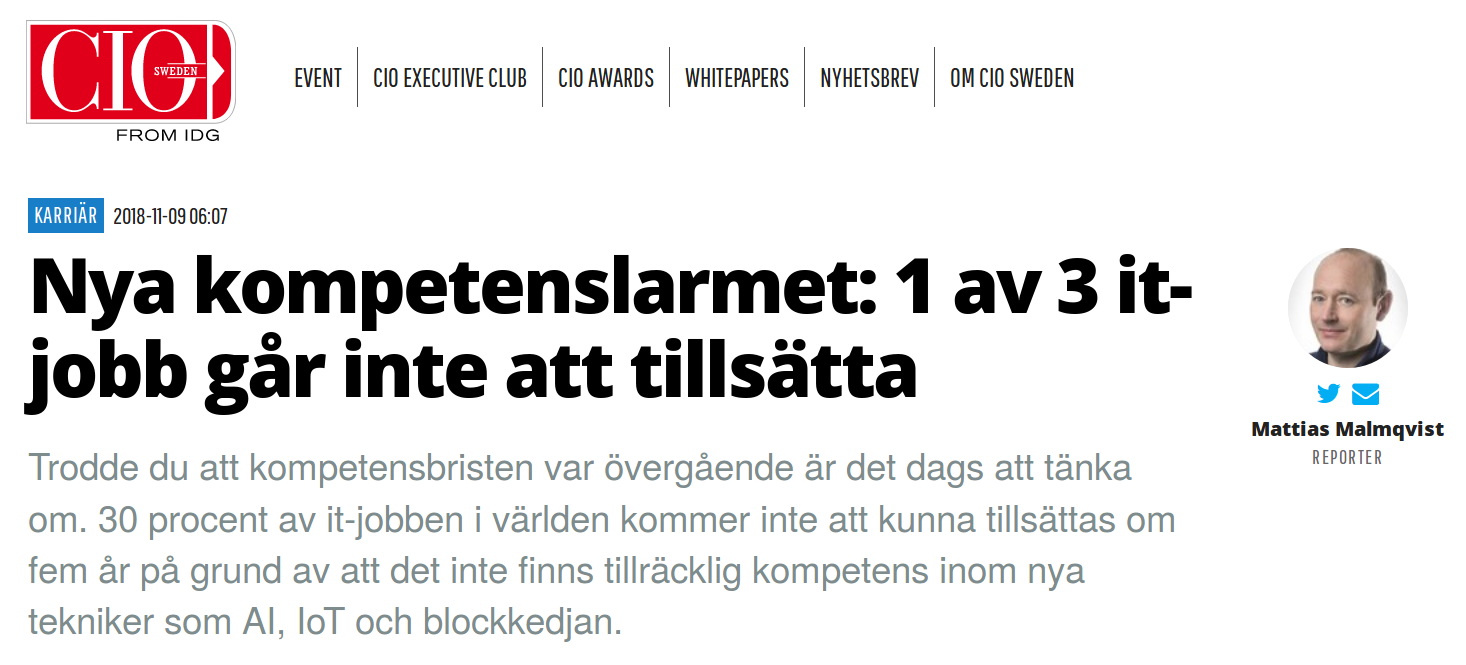
\includegraphics[height=0.75\textheight]{../../img/kompetenslarm-cio}
\end{Slide}

\begin{Slide}{Återkommande larm om kompetensbrist (2017)}
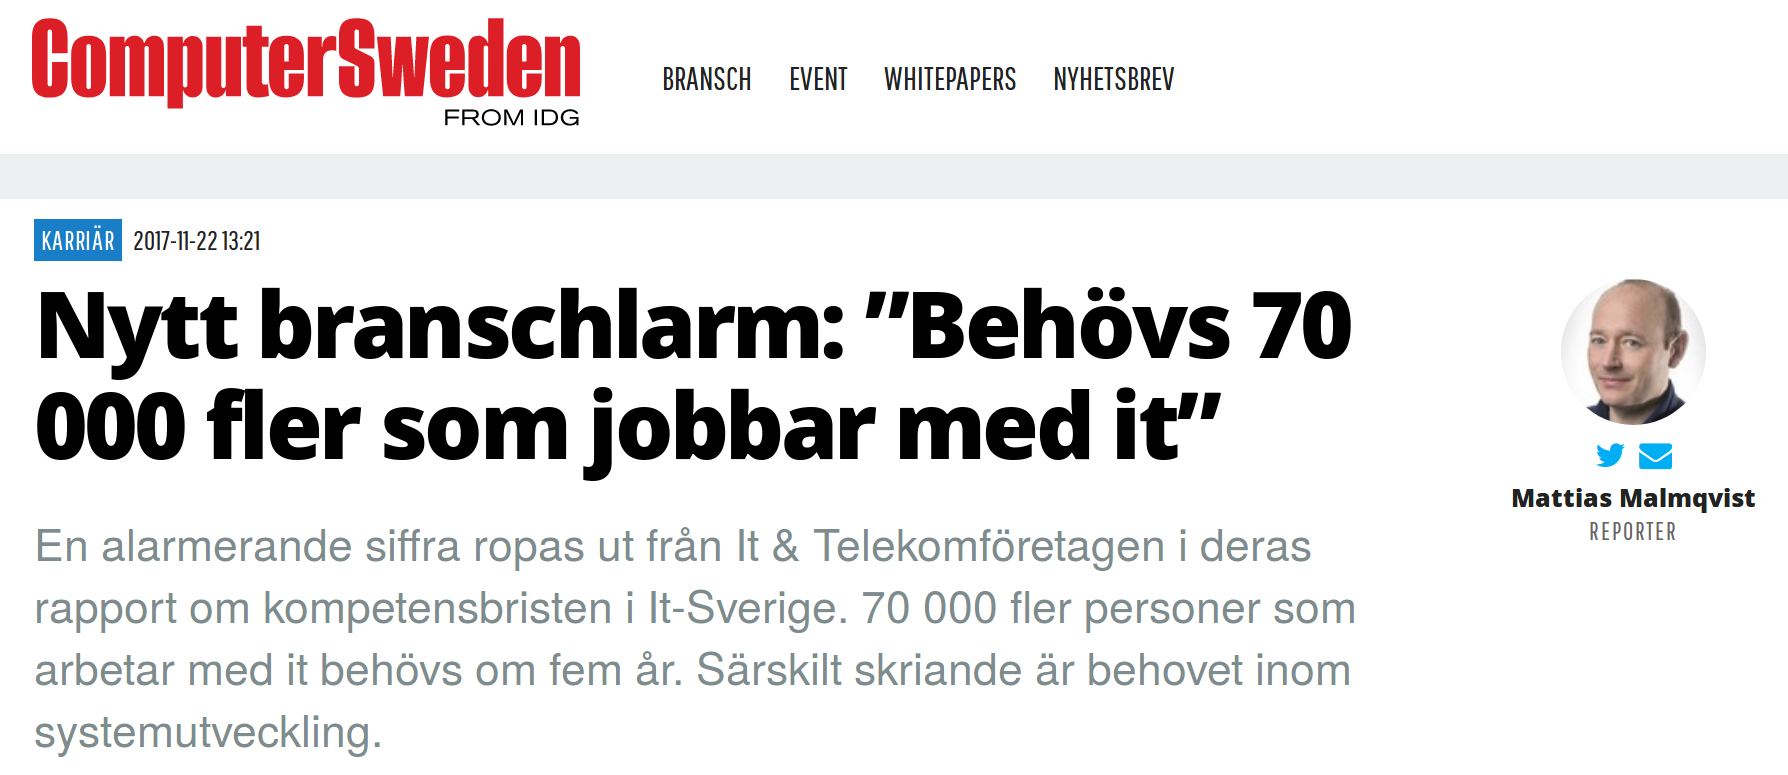
\includegraphics[height=0.75\textheight]{../../img/kompetenslarm-cs}
\end{Slide}




\begin{Slide}{Universiteten levererar inte (än)}
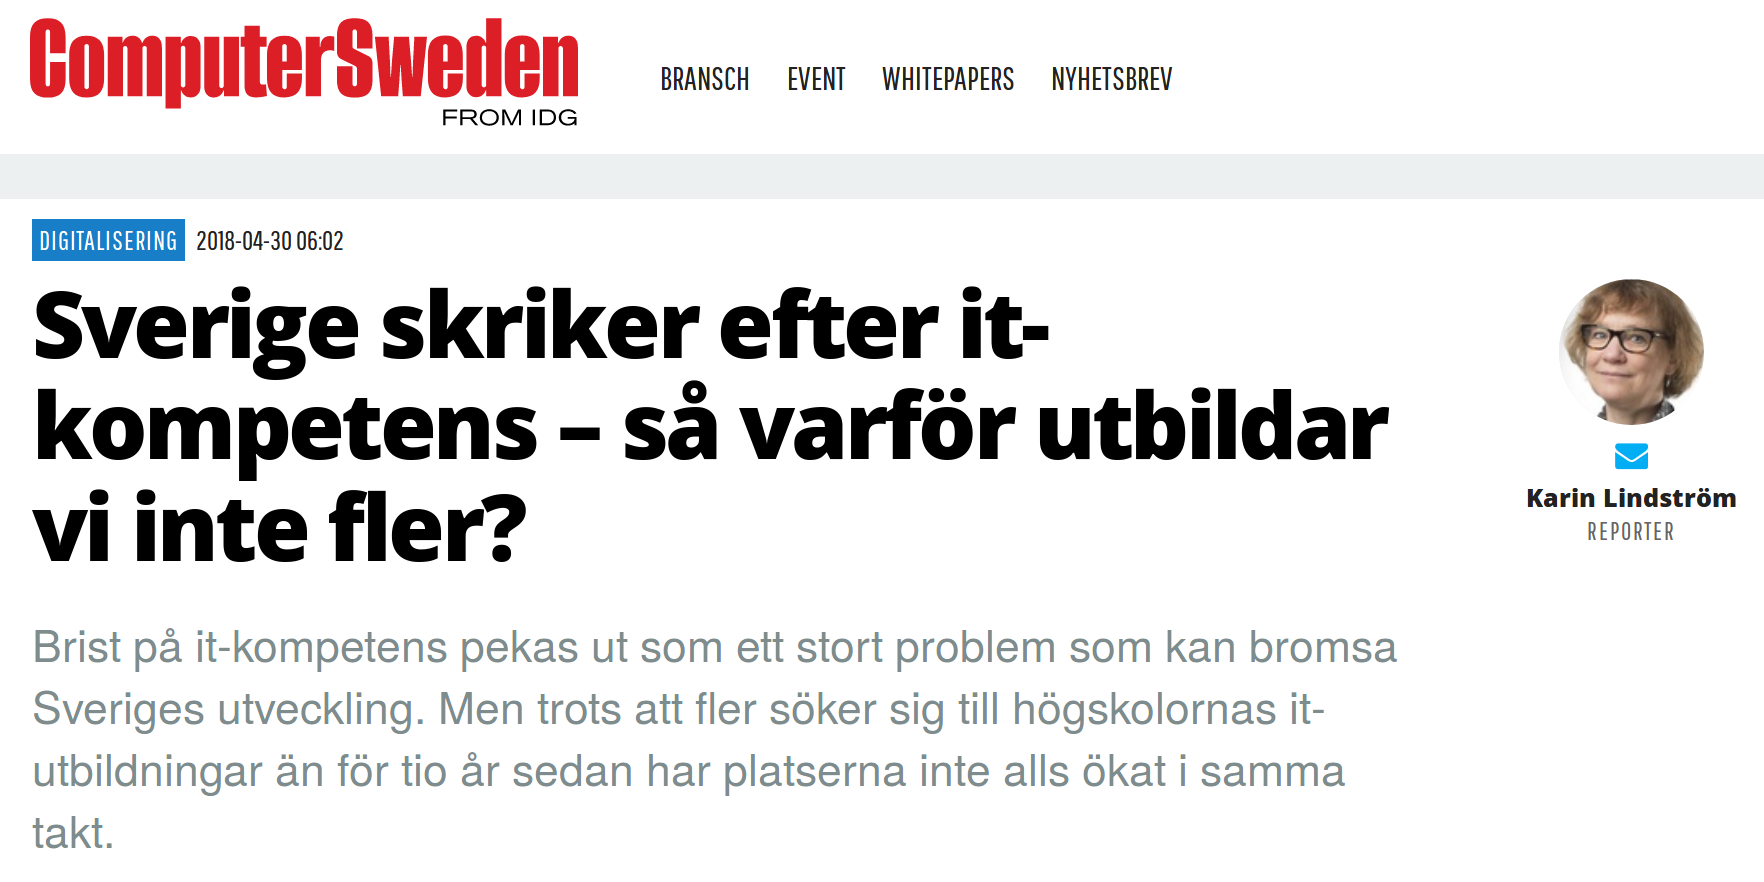
\includegraphics[height=0.75\textheight]{../../img/utbilda-fler}
\end{Slide}


\begin{Slide}{På gång på LTH: utveckling av undervisningen med anledning av samhällets digitalisering (1)}
  Urval av exempel på omfattande utveckling vid inst. f. \textbf{datavetenskap}: 
  \begin{enumerate}\footnotesize
    \item Ny professor Volker Kruger i robotik ht 2018. 
    \item Ny bitr. lektor Luigi Nardi i maskininlärning ht 2019. 
    \item Ny lektor Christoph Reichenbach i programvaruteknik vt 2018.
    \item Ny bitr. lektor Emma Söderberg i programvaruteknik vt 2018.
    \item Ny valfri kurs ''Tillämpad maskininlärning'' ht 2018. Enormt söktryck, 90 platser.
    \item Kursutveckling av ''Språkteknologi''. Nya moment om maskininlärning för naturligt språk.  Antalet studenter har dubblerats senaste åren. Cirka 150 deltagare i år.
    \item Kursutveckling av ''Artificiell intelligens'', nu på A-nivå. Antalet deltagare har dubblerats de senaste åren, från cirka 50 till 100 deltagare.
    \item Ny kurs ''Flertrådad programmering'', ht 2019, omfattande uppdatering av tidigare kurs.
    \item Ny kurs i ''Webbprogrammering'', vt 2019.
    \item Ny kurs i ''Intelligenta Autonoma System'', från 2020/21.
    \item Nytt masterprogram i ''Maskininlärning'', från 2020/21.
  \end{enumerate}
  Läs mer här: \url{http://cs.lth.se}
\end{Slide}

\begin{Slide}{På gång på LTH: utveckling av undervisningen med anledning av samhällets digitalisering (2)}
  Urval av exempel på omfattande utveckling vid inst. f. \textbf{elektro- och informationsteknik}: 
  \begin{enumerate}
    \item Ny kurs ''Konstruktion av säkra system'', med fokus på datasäkerhet och förståelse för förutsättningar för personlig integritet.
    \item Ny kurs i ''Högpresterande fibernät'', ger förståelse för bitöverföring från användarens access till nätet upp till kärnnäten, både för fix \& mobil anslutning.
    \item Kursutveckling av ''Internetprotokoll'', nytt projekt.
    \item Ny kurs ''Kretskortsdesign och prototypkonstruktion'', utvecklingen av prototyper, speciellt med inriktning mot IoT-enheter.
    \item Utveckling av labbar i för kurserna ''Datorteknik''  och ''Digitala system'', med fokus på hårdvarunära programmeringen och IoT-enheter. 
  \end{enumerate}
  Läs mer här: \url{http://www.eit.lth.se}
\end{Slide}





\begin{Slide}{Några strategiskt frågor för LTH}
  \begin{enumerate}\small
    \item Vad är viktigast att LTH:s nyexaminerade har lärt sig för att under ett livslångt yrkesliv kunna vara \textbf{kompetenta digitaliseringsagenter} inom samhällets alla sektorer? \\(Balans mellan djup IT-kunskap och djup domänkunskap.)
    \item Vilken balans mellan och inom olika program bör vi ha?
    \begin{enumerate}
      \item Ökad andel digitaliseringskompetens inom befintliga program? (Vad kan minskas?)
      \item Fler platser på IT-programmen? (Vilka program kan ha färre platser?)
    \end{enumerate}  
    \item Hur ska vi finansiera och utveckla \textbf{fortbildning} av yrkesverksamma?
    \item Hur ska vi finansiera och utveckla \textbf{omskolning} av arbetslösa?
    \item Hur ska vi finansiera och utveckla  \textbf{forskning och kompetensutveckling} av lärare?
    \item Vilken roll ska LTH ha vid Lunds universitet?
    \begin{enumerate}
      \item Hur får studenter vid \textbf{andra fakulteter} tillgång till digitaliseringskompetens?
      \item Hur får LTH-studenter bildning inom digitaliseringens etiska och politiska \textbf{ödesfrågor}?
    \end{enumerate}  
    \item Hur ska \textbf{digitaliseringen av pedagogiken} ske så att vi är relevanta och attraktiva även för morgondagens studenter?
  \end{enumerate}  
\end{Slide}


\begin{Slide}{LTH:s framtida konkurrenter?}
  \begin{minipage}{0.23\textwidth}
  \begin{itemize}
    \item Amazon
    \item Facebook
    \item Google
  \end{itemize}
  \end{minipage}
  \begin{minipage}{0.7\textwidth}
    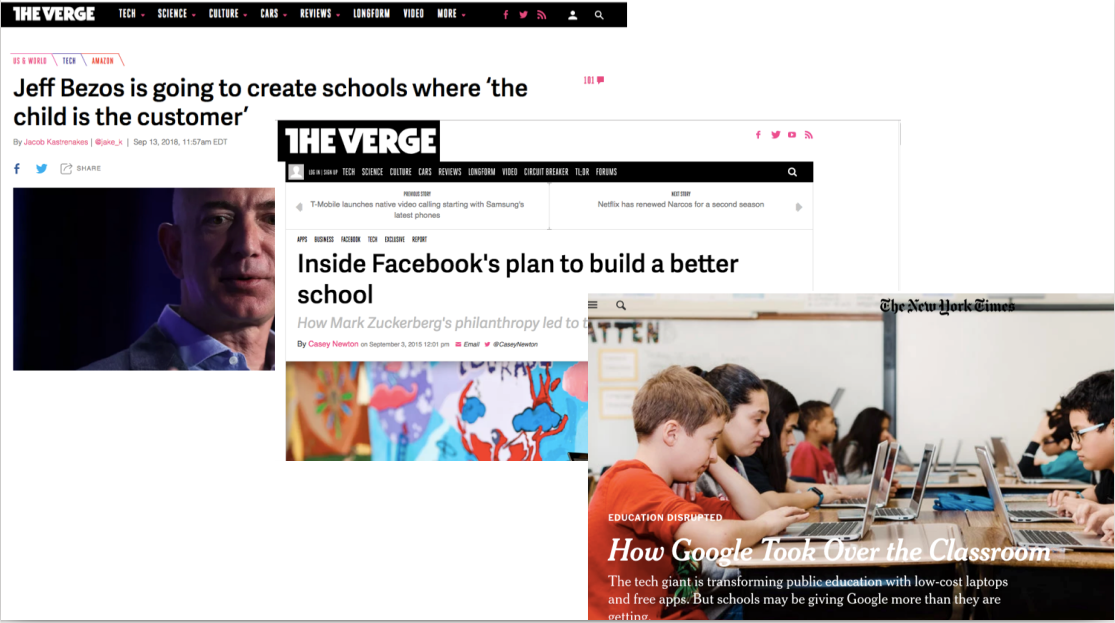
\includegraphics[height=0.85\textheight]{../../img/afg}
  \end{minipage}
\end{Slide}

\begin{frame}[plain]
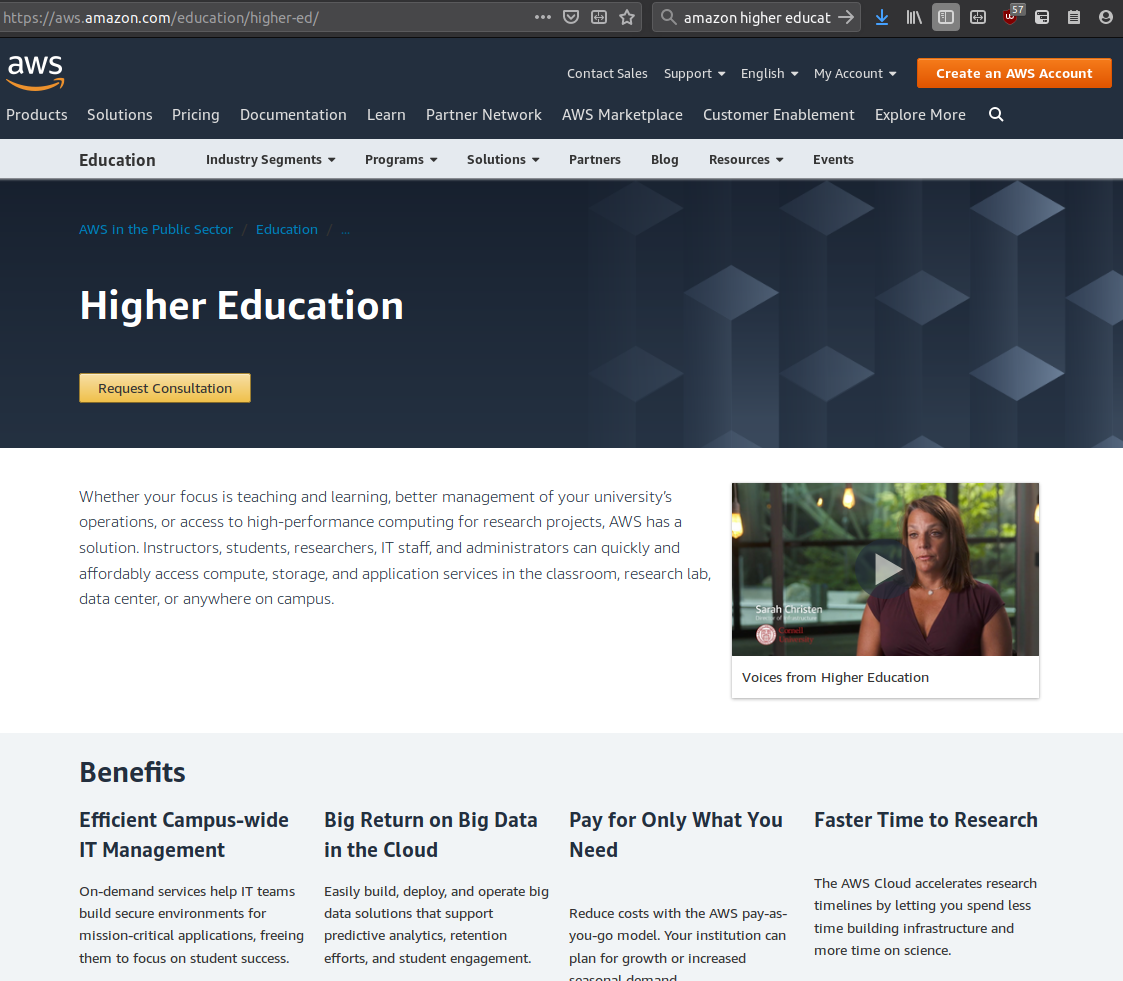
\includegraphics[height=1.3\textheight]{../../img/aws}
\end{frame}


\begin{Slide}{Exempel på input från näringslivet}
  Några axplock ur förslagen i rapport från Swedsoft: \\''Kan Sverige vara världsledande på mjukvaruutveckling och -forskning i framtiden?''\\
  \href{https://www.swedsoft.se/wp-content/uploads/sites/7/2019/09/Swedsoft-Helhetssyn-p\%C3\%A5-mjukvarans-betydelse-f\%C3\%B6r-digitalisering-och-konkurrenskraft.pdf}{www.swedsoft.se, 2019-09-04}
\begin{itemize}
  \item Det krävs ekonomiska förutsättningar för lärosätena att arbeta med yrkesverksamma.
  \item Nationellt kunskapslyft för att stimulera kompetenshöjningar, även på grundläggande högskolenivå och för personer med olika utbildningsbakgrund.
  \item Stipendier till utvalda mjukvaruutbildningar för utländska studenter, som garanteras att få stanna kvar i Sverige under en längre period efter utbildningen.
  \item Brett forskningsprogram inom mjukvaruutveckling där forskning sker i samverkan med företag, öppet för alla lärosäten med minst ett treårigt mjukvaruutvecklings- eller datavetenskapligt utbildningsprogram.
\end{itemize}
\end{Slide}




\section{Gruppdiskussioner}

\begin{Slide}{Gruppdiskussioner}
  \begin{itemize}
    \item Syfte: ge input till framtagandet av LTH:s digitaliseringsstrategi med fokus på grundutbildning och arbetet med att dimensionera och utforma innehållet i våra framtida yrkesexamina.
    \item Diskussionsfrågor: \\ 
    \item[] Hur påverkar digitaliseringen...

    \begin{enumerate}
        \item  ...era \textbf{produkter/tjänster/verksamheter} i
        närtid / på sikt?
        
        \item ...ert \textbf{behov av kompetens} i närtid / på
        sikt?
    \end{enumerate}

    \item Utse rapporteringsansvarig inom gruppen.
    \item Diskussionstid: 30 min
    \item Återrapporteringstid: 5 min per grupp
    \item Använd gärna blädderblock för att sammanfatta resultatet av diskussionen 
  \end{itemize}
\end{Slide}

\section{Avslutning}

\begin{Slide}{Hur använder LTH resultatet från idag?}
  \begin{itemize}
    \item LTH arbetar med framtagande av en strategi för digitalisering som omfattar:
    \begin{itemize}
      \item Grundutbildning
      \item Forskning och forskarutbidlning
      \item Samverkan
      \item Infrastruktur och stöd
    \end{itemize}
    \item LTH:s digitaliseringsutredning pågår under 2019 och alla våra intressenter är välkomna att bidra med bedömning av framtida behov och prioriteringsunderlag.
    \item Input från näringslivsrådet och andra intressenter kommer att redovisas för LTH:s styrelse och utgöra underlag för kommande rektorsbeslut. 
    \item Kontakta LTH:s vicerektor för digitalisering: \url{bjorn.regnell@cs.lth.se}
  \end{itemize}
  
\end{Slide}

\end{document}